\section{扩展知识:\texorpdfstring{$y=x+\frac{1}{x}$}{y=x+1/x}的图形}

本节我们绘制
\[
y=ax+\frac{b}{x}
\]
的图形,以加深对基本不等式的理解。

~

由于函数是奇函数,且$x\ne 0$,所以我们只绘制$x>0$部分,先从最基本的开始,如下函数:
\[
y=x+\frac{1}{x} \qquad x>0
\]
图形如下,不难发现:
\begin{itemize}
    \item 图形由两部分组成,左边是$\frac{1}{x}$主导,右边是$x$主导;
    \item $y$先减小后增大,当$x=1$时取最小值2;
    \item $x=0$和$y=x$是函数的两条渐近线。
\end{itemize}

\begin{figure}[h]
\centering
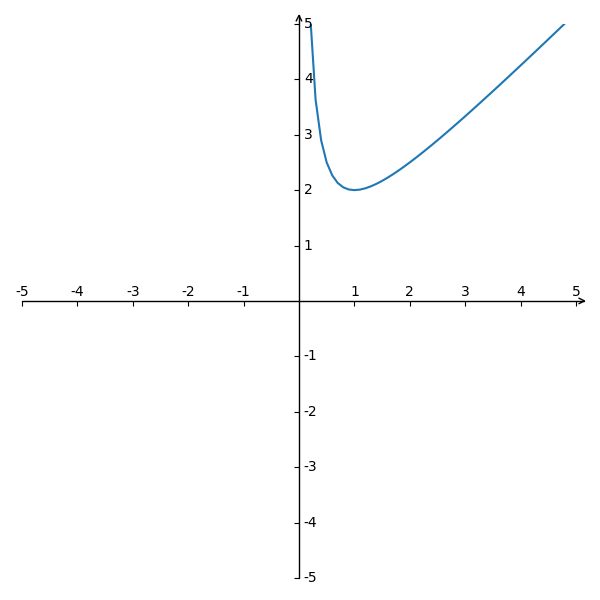
\includegraphics[height=6cm]{2.4-1.png}
\end{figure}

~

若我们调整$a$
\begin{align*}
&y=0.5x+\frac{1}{x} \\
&y=x+\frac{1}{x} \\
&y=2x+\frac{1}{x}
\end{align*}
则函数图形如下。

\begin{figure}[ht]
\centering
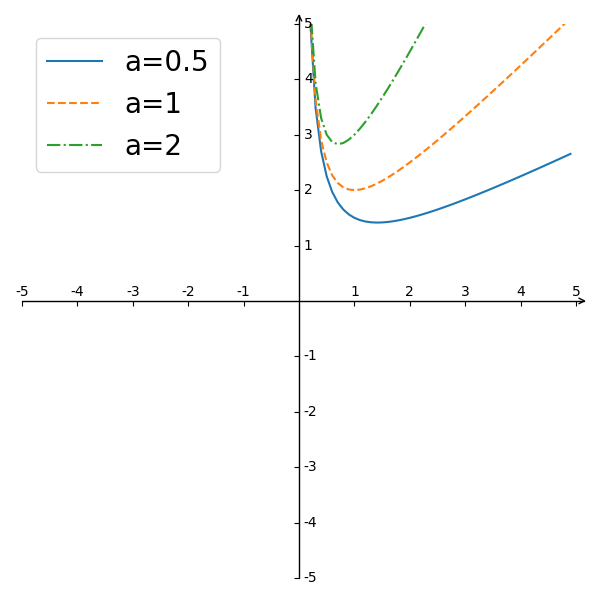
\includegraphics[height=6cm]{2.4-2.png}
\end{figure}

~

若我们调整$b$
\begin{align*}
&y=x+\frac{0.5}{x} \\
&y=x+\frac{1}{x} \\
&y=x+\frac{2}{x}
\end{align*}
则函数图形如下。

\begin{figure}[h]
\centering
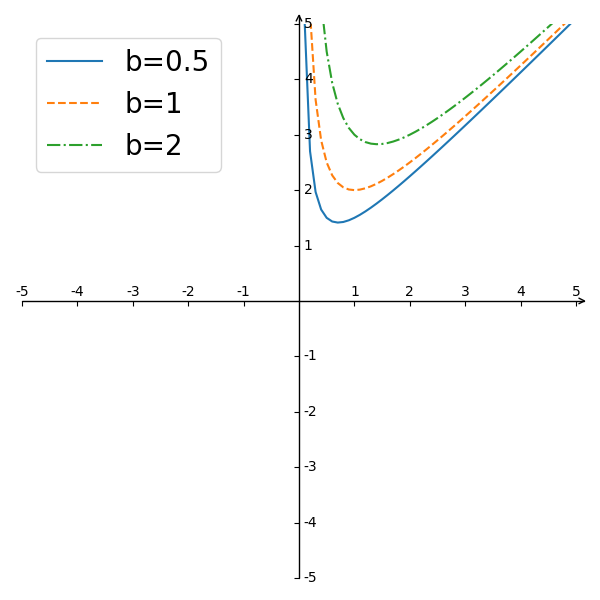
\includegraphics[height=6cm]{2.4-3.png}
\end{figure}

不难发现:
\begin{itemize}
    \item 调节$a$,影响的是$x$部分,图象上反映在右侧变化较大;
    \item 调节$b$,影响的是$1/x$部分,图象上反映在左侧变化较大;
    \item 无论调节$a$还是$b$,最值都会发生变化。
\end{itemize}




